\chapter{Implementation}

% organise by features of app/api or by stages?

\section{Overview}

Since the back-end API and front-end mobile app are so tightly connected, implementing them linearly would not be logical as errors between the app and server will not be detected as quickly and requirements of features may change over time. I therefore implemented the two in parallel, normally a feature at a time, so that a working implementation for each subsequent feature was produced at the end of each iteration.

This section splits the implementation into the two sections, API and mobile app, with each discussing the features implemented chronologically.

\section{API}

\subsection{Endpoint Routing}

To set up endpoints on the API to respond to client requests, the popular Express web framework ***ref*** was used. Express's router object determines how the API handles a request to a certain URI with a specific HTTP method.

The main file loaded when a request is made, \texttt{app.js}, specifies the main endpoint for the API and links this endpoint to an Express router. This router specifies the path for each of the main API routes, following the design from Figure \ref{fig:api-routes} in the previous section. Each path contains a router which matches each of the endpoints it serves as well as a controller containing functions which are executed when a router endpoint is matched from a request. An example of how a request to login a user is routed through the API is shown in Figure ***.

\subsection{Authentication}



\subsection{Querying Database}

% mention mongoose populate

\subsection{Storing Images} \label{implementation:storing-images}

% maybe move this to design and move file storage design section to background?

There are two methods that can be used when uploading images via an API to a file storage service such as AWS S3. The first of which is direct upload where the client -- the mobile app in this case -- uploads the file directly to S3, bypassing the API altogether. The other option, known as pass-through upload, is to upload the image via a request to the API and then let the API handle the upload to S3. The former of the two options is the most commonly used since it does not require any extra processing to be performed by the API, which could result in slower response times especially on Heroku.

While the direct upload method does also require a slightly more complicated implementation, I decided to choose it based on the needs of this project and its ability to be scaled effectively.

% implementation from here

Having chosen to use the direct upload method described in Section \ref{subsection:file-storage-methods}, I outlines the steps that needed to be followed when uploading a file:

\begin{enumerate}[label=\textbf{Step \arabic*}]
  \item Request a pre-signed URL from the API to upload a file using the AWS SDK, giving the client the necessary permissions to upload at that location.
  \item Upload the file directly from the client to the URL.
  \item Store a reference to the URL where the file is stored either locally or in the back-end so that it can be accessed in the future.
\end{enumerate}

Even though the only current use for the file upload capability in the app is to store the thumbnail images of tracked walks, I wanted to make the code as re-usable as possible so that any feature implemented in the future could upload files with ease.

To implement \textbf{Step 1}, I created an endpoint in the API at \texttt{/walks/create/upload} to retrieve a signed URL from AWS S3. This accepted a GET request with no parameters that returned a URL that would expire in 60 seconds. The expiry time was used so that numerous empty URLs were not created by continuously sending a \texttt{GET /walks/create/upload} request, while still allowing enough time for the file to be uploaded by the client.

% alamofire or apimanager is not refd here
% move communication with API section to before this one?

Upon receiving the URL from the API, the mobile app then uploads the file to this location as in \textbf{Step 2}. Alamofire provides an \texttt{upload()} method along with its \texttt{request()} method that supports sending of larger amounts of data such as a file. The method accepts the file as a parameter in \texttt{Data} format, a datatype commonly used throughout iOS to store and transfer files or objects. Images can be converted to their Data representation using the \texttt{UIImageJPEGRepresentation()} function declared in Apple's UIKit, passing in a native \texttt{UIImage} object.

While the previous two steps have been fairly general to upload a file, \textbf{Step 3} of the method is what applies this code to the feature being implemented. In the case of this project, I needed to upload an image of a tracked walk and store a reference to the URL of that image in its own Walk document in the database. Once the image has been uploaded successfully, a Walk document is created via sending a \texttt{POST /walks/create} request to the API. The parameters of that request include the name of the walk, an array of coordinates and the URL of the image that was uploaded in the previous step.

\section{Mobile App}

\subsection{Communication with API}

To handle requests from the multiple APIs used within the mobile application, a singleton class \texttt{APIManager} was used that was accessible throughout the app to organise each API call. The main function of \texttt{APIManager} was to abstract the network requests through the HTTP networking library Alamofire ***ref*** -- a more elegant way to handle networking in comparison to Swift's default network tools, providing simple JSON encoding and serialisation as well as response validation.

Alamofire's Router design pattern allowed me to define a complete set of paths, methods and parameters needed for the endpoints of a particular API and hence construct a request with with any HTTP headers as appropriate. The Router was implemented as a protocol containing the necessary fields that needed to be overridden, and each API that needed to be documented in this way adopted this protocol and used an enumeration pattern to define each of the available endpoints for that API. The specific endpoint case for a given API router would then be passed as a parameter to Alamofire's \texttt{request()} method, which would construct and send the HTTP request as necessary.

Finally, an enumeration was created to represent the success or failure response received from the API. Enumeration cases in Swift can contain parameters and so I defined the success response to contain a JSON object that contained the response from the API, constructed in Alamofire's asynchronous request callback. Meanwhile, the failure case contained a Swift error object whose error code and description were populated from the information received from the API. Figure \ref{fig:api-communication} explains in more detail the path of method calls and how data is passed through callbacks when making a network request.

\begin{figure}[hbt]
  \centering
  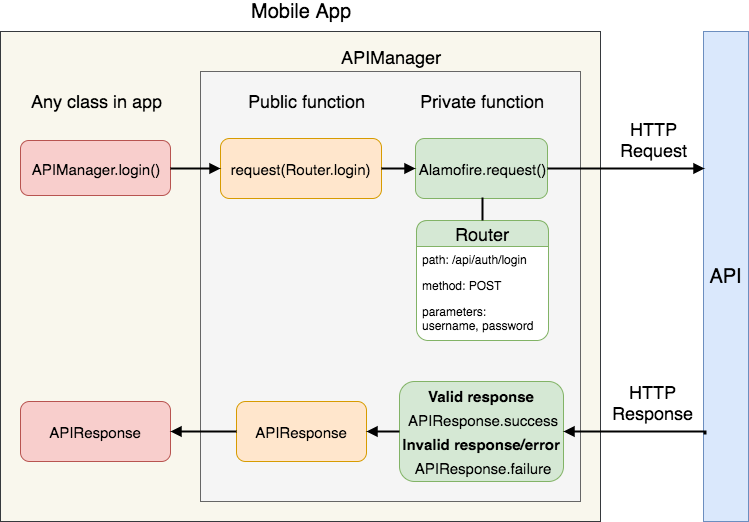
\includegraphics[width=\textwidth]{api-communication}
  \caption{The path of method calls and callbacks used when making a network request within the mobile app, namely logging the user in. The top row of arrows represent method calls being made from the app whilst the bottom row of arrows represent the callbacks for each method once the network response is received.}
  \label{fig:api-communication}
\end{figure}


\subsection{Points of Interest}

\subsection{Gamification} \label{subsection:gamification}

% should this be in mobile app section?

\subsection{Walk invitations}

\section{Challenges}